% Part: sets-functions-relations
% Chapter: infinite
% Section: hilberts-hotel
%
\documentclass[../../../include/open-logic-section]{subfiles}

\begin{document}

\olfileid{sfr}{infinite}{hilbert}
\olsection{ہلبرٹ دا ہوٹل}

قدرتی عدداں دا سیٹ صاف طور تے لامتناہی اے۔ سو جے اسی قدرتی عدداں نوں
\emph{پہلے توں من} نہیں لینا چاہندے، تاں ساڈا پہلا قدم لامتناہی سیٹ
دی خاصیت ایسے لفظاں وچ دَسنا ہونا چاہیدا اے جیہناں وچ خود قدرتی عدداں
دا ذکر ضروری نہ ہووے۔ ہلبرٹ نے 1924 دے اک لیکچر وچ اک سوہنا طریقہ
پیش کیتا۔ اوہ سانوں ایہ تصور کرن نوں آکھدا اے:
% PNBINF-001 ماخذ دی درستی: ”our first step must be characterize“ وچ مصدر دا نشان رہ گیا سی؛ ایتھے پہلا قدم خاصیت دَسنا آکھیا اے۔
\begin{quote}
[\ldots] اک ایسا ہوٹل جیہدے وچ کمراں دی متناہی گنتی اے۔ ایہناں
سارے کمراں وچ عین اک اک مہمان ٹھہریا ہووے۔ جے ہُن مہمان کسے طرح آپس
وچ کمرے بدل لَین، [پر] ایس طرح کہ ہجے وی ہر کمرے وچ اک توں ودھ بندہ
نہ ہووے، تاں کوئی کمرہ خالی نہیں ہووے گا، تے ہوٹل دا مالک ایس طریقے
نال نویں آؤندے مہمان لئی نویں تھاں نہیں بنا سکدا [\ldots
\textparagraph \ldots]

ہُن اسی مقرر کردے آں کہ ہوٹل دے نمبر لگے لامتناہی کمرے $1$، $2$،
$3$، $4$، $5$، \dots، ہون، تے ہر کمرے وچ عین اک مہمان ٹھہریا ہووے۔
جیویں ای کوئی نواں مہمان آوے، مالک نوں صرف ہر پرانے مہمان نوں اوس
کمرے وچ بھیجنا اے جیہدا نمبر اک ودھ اے، تے کمرہ~$1$ نویں آؤندے مہمان
لئی خالی ہو جاوے گا۔
	\begin{center}
		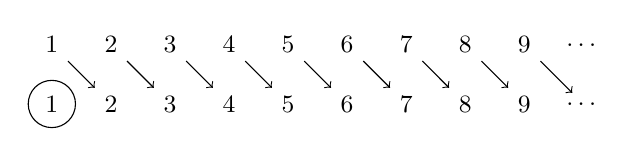
\begin{tikzpicture}[scale = .75]
		\foreach \x in {1, 2, 3, 4, 5, 6, 7, 8, 9}
		{
			\node (\x a) at (\x, 1) {\small{\x}};
			\node (\x b) at (\x, 2) {\small{\x}};
		}
		\node (dotsa) at (10, 1) {\small{\ldots}};
		\node (dotsb) at (10, 2) {\small{\ldots}};
		\draw[->] (1b)--(2a);
		\draw[->] (2b)--(3a);
		\draw[->] (3b)--(4a);
		\draw[->] (4b)--(5a);
		\draw[->] (5b)--(6a);
		\draw[->] (6b)--(7a);
		\draw[->] (7b)--(8a);
		\draw[->] (8b)--(9a);
		\draw[->] (9b)--(dotsa);
		\draw (1,1) circle (.4);
		\end{tikzpicture}
	\end{center}
	(\citealt[730]{EwaldSieg2013} وچ چھپیا؛ ماخذ مصنفا دا ترجمہ)
\end{quote}
بنیادی نکتہ ایہ اے کہ ہلبرٹ دے ہوٹل وچ لامتناہی کمرے نیں؛ تے اسی
اوہدی سمجھاوت نوں ایس گل دے معنی دی تعریف سمجھ سکدے آں۔ اصل وچ ایہ
ڈیڈیکائنڈ دا طریقہ سی (بے شک ایتھے ایہنوں بہت وڈے زمانوی اُلٹ پھیر نال
پیش کیتا گیا اے؛ ڈیڈیکائنڈ دی تعریف \citeyear{Dedekind1888} دی اے):

\begin{defn}\ollabel{defn:DedekindInfinite}
سیٹ $A$ \emph{ڈیڈیکائنڈ لامتناہی} اُدوں تے صرف اُدوں اے جدوں $A$ توں
$A$ دے اک حقیقی ذیلی سیٹ ول کوئی !!a{injection} ہووے۔ یعنی کوئی
$o \in A$ تے !!a{injection} $f \colon A \to A$ ہووے جیہدے لئی
$o \notin \ran{f}$۔
\end{defn}

\end{document}
